\documentclass{article}
\usepackage[utf8]{inputenc}
\usepackage{amssymb,amsmath}
\usepackage[usenames, dvipsnames]{color}
\usepackage{amsthm}
\textheight=24cm % высота текста
\textwidth=15cm % ширина текста
\oddsidemargin=1.0cm % отступ от левого края
\topmargin=-1.5cm % отступ от верхнего края
\parindent=24pt % абзацный отступ
\parskip=0pt % интервал между абзацами
\tolerance=2000 % терпимость к "жидким" строкам
\flushbottom % выравнивание высоты страниц
\newtheorem{theorem}{Theorem}

\title{Representations of flat virtual braids which do not preserve the forbidden relations}
\author{B.~Chuzhinov \and I.~Emelianenkov \and  M.~Ivanov \and E.~Markhinina  \and S.~Panov \and  T.~Plevako \and N.~Singh \and S.~Vasyutkin \and V.~Yakhin \and V.~Bardakov \and A.~Vesnin \and T.~Nasybullov} 
\date{July 2020}
\usepackage{natbib}
\usepackage{graphicx}

\begin{document}
\maketitle
\begin{abstract}
 Short formulation of all our results.
 
 
 ~\\
 \textit{Keywords:}
 
 ~\\
 \textit{Mathematics Subject Classification:} 
\end{abstract}

\section{Introduction}
Motivation here: knot theory, flat virtual knots, braids, flat virtual braids, representations of braid groups, question of Bardakov from \cite{problems}

Everyone comes across knots. For example, everybody knows about shoelace knots, neck tie knots, knots in logos. 

To understand what is the mathematical knot imagine one experiment. Take a long rope, tangle it and glue the ends. This is a mathematical knot. In mathematical term mathematical knot is  a closed curve in the Euclidean space $R^3$. \\

A link is two or more knots which may or may not be entangled.

Two knots/links are called equivalent if one can be deformed into other by wiggling the knot in $R^3$. The knots are allowed to stretch, shrink and twist but not allowed to cross themselves.

One of the basic problems of the knot theory is the problem of determining by two given links equivalent they are or not.\\

Leaning braid helps us to study knots. Braids on $n$ threads are a set of  $n$ threads entangled with each other which connect $n$ points on one straight line with $n$ points on a parallel straight line.(image)

Braids on $n$ strands can be multiplied with each other. The multiplication $\alpha\beta$ of the braid $\alpha$ on $n$ strands with the braid $\beta$ on $n$ strands is the braid $\alpha$ obtained from the braid $\beta$  by adding braid $\beta$ to it from below. (image)

So the set of all braids on $n$ strands with the multiplication operation defined in this way forms a group, which is denoted by the symbol $B_n$ and is called a braid group on $n$ strands.

In mathematical term, a braid group $B_n$ is a group with generators $\sigma _1,\sigma _2,\dots,\sigma _{n-1}$ and defining relations 

\begin{align*}
\sigma _i\sigma _{i+1}\sigma _i &= \sigma _{i+1}\sigma _i\sigma _{i+1}&&i = 1, 2, \dots. n-2\\
\sigma _i\sigma _j &= \sigma _j\sigma _i&&|i-j|\geqslant   2\\
\end{align*}


Braids are objects closely related to knots. If $\alpha$ is a braid on $n$ strands, then to connect the first upper point to the first bottom point, the second upper braid point to the second bottom braid point, and so on we get some link $\check  \alpha$ (image).

For every link $K$ exists some braid $\alpha$, where link $K$ and $\check  \alpha$ are equivalent.\\


The group of flat virtual braids on $n$ strands is the group $FVB_n$ with generators  $\sigma _1,\sigma _2,\dots,\sigma _{n-1}\rho_1,\rho _2,\dots,\rho _{n-1}$ and defining relations 

\begin{align*}
\sigma_i^2&=1 && i = 1, 2, \dots,n-1,\\
\sigma_i\sigma _{i+1}\sigma _i &= \sigma _{i+1}\sigma _i\sigma _{i+1}&& i = 1, 2, \dots. n-2, \\
\sigma _i\sigma _j &= \sigma _j\sigma _i && |i-j|\geqslant   2,\\
\rho_i^2&=1 &&i = 1, 2, \dots,n-1, \\
\rho_i\rho _{i+1}\rho _i &= \rho _{i+1}\rho_i\rho _{i+1} &&i = 1, 2, \dots. n-2,\\
\rho _i\rho _j &= \rho _j\rho _i && |i-j|\geqslant 2,\\
\sigma _i\rho _j &= \rho _j\sigma _i &&|i-j|\geqslant   2,\\
\rho_i\rho _{i+1}\sigma _i &= \sigma _{i+1}\rho_i\rho _{i+1} && i = 1, 2, \dots. n-2.\\
\end{align*}

Our aim is construct a representation $FVB_n \rightarrow Aut (G)$, where $G$ is some "good" group, for example, a free group.

\section{Preliminaries}
Definition of $FVB_n$ (or all braid groups smoothly going to flat virtual braids)

Explanation what is $FVP_n$

Explanation that $FVB_n=FVP_n\rtimes S_n$

Description of $FVP_3$ from \cite{BarBelDom}

Known representations of $FVB_n$ and why they are bad for us.

Group $FVB_n$ is linear \cite{BarBelDom}
\section{New representation}

Consider a free group $F_{2n}=\langle x_1, x_2,\ldots , x_n, y_1, y_2, \ldots , y_n \rangle$. M.~Ivanov and I.~Emelianenkov suggested the mapping $\theta_n:FVB_n \rightarrow Aut(F_{2n})$, which acts on the generators as follows:
$$
\theta_n(\sigma_i):
\begin{cases}
x_i \rightarrow x_{i+1}y_{i+1},\\
x_{i+1} \rightarrow x_iy_{i+1}^{-1},\\
\end{cases},\quad
\theta_n(\rho_i):
\begin{cases}
x_i \rightarrow x_{i+1},\\
x_{i+1} \rightarrow x_i,\\
y_i \rightarrow y_{i+1},\\
y_{i+1} \rightarrow y_i,\\
\end{cases}
$$

The main result of this section is the following

\begin{theorem}
The mapping $\theta_n:FVB_n \rightarrow Aut(F_{2n})$ as defined above is representation of flat virtual braids which do not preserve the forbidden relations.
\end{theorem} 

\begin{proof}
To show that $\theta_n$ is representation sufficinatly check that images of generators satisfy the relations (?). Denote by $s_i$ and $r_i$ images of $\sigma_i$ and $\rho_i$ respectively. Agree to understand the composition $sr$ of mappings $s$ and $r$ as sequential action first $s$ then $r$.

It is not hard to see that $s_is_j=s_js_i$, $r_ir_j=r_jr_i$ and $s_ir_j=r_js_i$ for $|i-j|\ge2$. Indeed, automorphisms $s_i$ and $r_i$ do not act identically only on $x_i, x_{i+1}, y_i, y_{i+1}$. Then for $|i-j|\ge2$  $s_i$ acts identically on  $x_j, x_{j+1}, y_j, y_{j+1}$ and $s_j$ acts identically on  $x_i, x_{i+1}, y_i, y_{i+1}$. Therefore $s_is_j=s_js_i$. Similarly with the equalities $r_ir_j=r_jr_i$ and $s_ir_j=r_js_i$ for $|i-j|\ge2$.

The calculations below prove that the remaining relations of flat virtual braids' group hold, and thus it is proved that $\theta_n$ -- representation.
$$
s_is_{i+1}s_i:
\begin{cases}
x_i\rightarrow x_{i+2}y_{i+2}y_{i+1}\\
x_{i+1}\rightarrow x_{i+1}\\
x_{i+2}\rightarrow x_iy_{i+1}^{-1}y_{i+2}^{-1}\\
\end{cases}, \quad
s_{i+1}s_is_{i+1}:
\begin{cases}
x_i\rightarrow x_{i+2}y_{i+2}y_{i+1}\\
x_{i+1}\rightarrow x_{i+1}\\
x_{i+2}\rightarrow x_iy_{i+1}^{-1}y_{i+2}^{-1}\\
\end{cases} 
$$

$$
r_ir_{i+1}r_i:
\begin{cases}
x_i\rightarrow x_{i+2}\\
x_{i+1}\rightarrow x_{i+1}\\
x_{i+2}\rightarrow x_i\\
y_{i} \rightarrow y_{i+2}\\
y_{i+1} \rightarrow y_{i+1}\\
y_{i+2} \rightarrow y_{i}\\
\end{cases} , \quad
r_{i+1}r_ir_{i+1}:
\begin{cases}
x_i\rightarrow x_{i+2}\\
x_{i+1}\rightarrow x_{i+1}\\
x_{i+2}\rightarrow x_i\\
y_{i} \rightarrow y_{i+2}\\
y_{i+1} \rightarrow y_{i+1}\\
y_{i+2} \rightarrow y_{i}\\
\end{cases} 
$$

$$
r_{i+1}r_is_{i+1}:
\begin{cases}
x_i\rightarrow x_{i+2}y_{i+2}\\
x_{i+1}\rightarrow x_{i+1}y_{i+2}^{-1}\\
x_{i+2}\rightarrow x_iy_{i+1}^{-1}\\
y_{i} \rightarrow y_{i+1}\\
y_{i+1} \rightarrow y_{i+2}\\
y_{i+2} \rightarrow y_{i}\\
\end{cases}, \quad
s_ir_{i+1}r_i:
\begin{cases}
x_i\rightarrow x_{i+2}y_{i+2}\\
x_{i+1}\rightarrow x_{i+1}y_{i+2}^{-1}\\
x_{i+2}\rightarrow x_iy_{i+1}^{-1}\\
y_{i} \rightarrow y_{i+1}\\
y_{i+1} \rightarrow y_{i+2}\\
y_{i+2} \rightarrow y_{i}\\
\end{cases} 
$$

Finally $r_is_{i+1}s_i(x_{i+2})=x_iy_{i+1}^{-1}y_{i+2}^{-1}$ but $s_{i+1}s_ir_{i+1}(x_{i+2})=x_iy_{i+2}^{-1}y_{i+1}^{-1}$. Also $r_{i+1}s_is_{i+1}(x_i)=x_{i+2}y_{i+2}y_{i+1}$ but $s_is_{i+1}r_i(x_i)=x_{i+2}y_{i+2}y_i$. Thus $\theta_n$ do not preserve the forbidden relations.    
\end{proof}

Remark that it solves the problem of V.~Bardakov from \cite{problems}
\section{What is the kernel}
Introduce the element from the kernel which we already have

Prove that this element is not trivial (use the discription of $FVP_3$ and express this element in terms of $a,b,c$)

Introduce the group $H$

The mapping $\theta$ acts on $a, b$ and $c$ in the following way:
$$
\theta(a) = \alpha : 
\begin{cases}
	x_1 \rightarrow x_1 y_3^{-1}\\
	x_2 \rightarrow x_2 y_1^{-1}\\
	x_3 \rightarrow x_3 y_3 y_1\\
	y_1 \rightarrow y_3\\
	y_2 \rightarrow y_1\\
	y_3 \rightarrow y_2
\end{cases},
\theta(b) = \beta :
\begin{cases}
	x_1 \rightarrow x_1\\
	x_2 \rightarrow x_2 y_3^{-1}\\
	x_3 \rightarrow x_3 y_3\\
	y_1 \rightarrow y_1\\
	y_2 \rightarrow y_3\\
	y_3 \rightarrow y_2
\end{cases},
\theta(c) = \gamma :
\begin{cases}
	x_1 \rightarrow x_1 y_1\\
	x_2 \rightarrow x_2 y_1^{-1} y_3^{-1}\\
	x_3 \rightarrow x_3 y_3\\
	y_1 \rightarrow y_2\\
	y_2 \rightarrow y_3\\
	y_3 \rightarrow y_1
\end{cases}.
$$

Proposition ${\rm ker}\cap H=1$. 

Proof. An arbitrary element in $\theta(H)$ has the form $\alpha^r \gamma^s = (\alpha \gamma)^r \gamma^{s-r}$ for some $r,s \in \mathbb{Z}$. It is easy to see that
$$
(\alpha \gamma)^r :
\begin{cases}
	x_1 \rightarrow x_1\\
	x_2 \rightarrow x_2 (y_1 y_3 y_1)^{-r}\\
	x_3 \rightarrow x_3 (y_3 y_1 y_2)^r\\
	y_1 \rightarrow y_1\\
	y_2 \rightarrow y_2\\
	y_3 \rightarrow y_3
\end{cases}.
$$

It means that $s-r = 0$, because in any other way $(\alpha \gamma)^r \gamma^{s-r} (x_1) \neq x_1$. But if $s-r = 0$, then for any $r \neq 0$ $(\alpha \gamma)^r (x_2) \neq x_2$. So, $r = 0 \Rightarrow s = 0 \Rightarrow \theta(H) \cap \ker \theta = \{id\}$.  

Here we understood that every element from $H$ can be written as $a^rc^s=(ac)^rc^{s-r}$, then we understood $ac$ fixes $x_1$, and $c^{s-r}$ fixes $x_1$ only when $s=r$, so, we moved to the element $(ac)^r$. After it we looked to all degrees of $(ac)^r$ and realized that it can go to the identical map only when $r=1$. 

Here write all the degrees of $a,b,c$.
\section{Linear representation}
Introduce the linear representation we got from our representation by automorphisms.

Note that the group $FVB_n$ is linear (it is know fact).

Is it true that the linear representation has the same kernel as representation by automorphisms?

\section{Representations of gauss virtual braids}
Let us go down and adopt these representations to the Gauss virtual knot theory.

Here we can easily find the kernel

Reduce the degree of representation.
\section{Knot theory}
Can we apply it to knot theory?

Explain why cannot we directly apply it to the knot theory.

Can we do something exotic to apply it somehow to knot theory?

\section{Questions}
Is the closure of the braid from the kernel trivial?

Look to the closure of $(\rho_1\sigma_2)^3$. Is the closure of this braid trivial?

Look to the other representations. Are they representations? Does our element belong to the kernel?

\begin{enumerate}
    \item 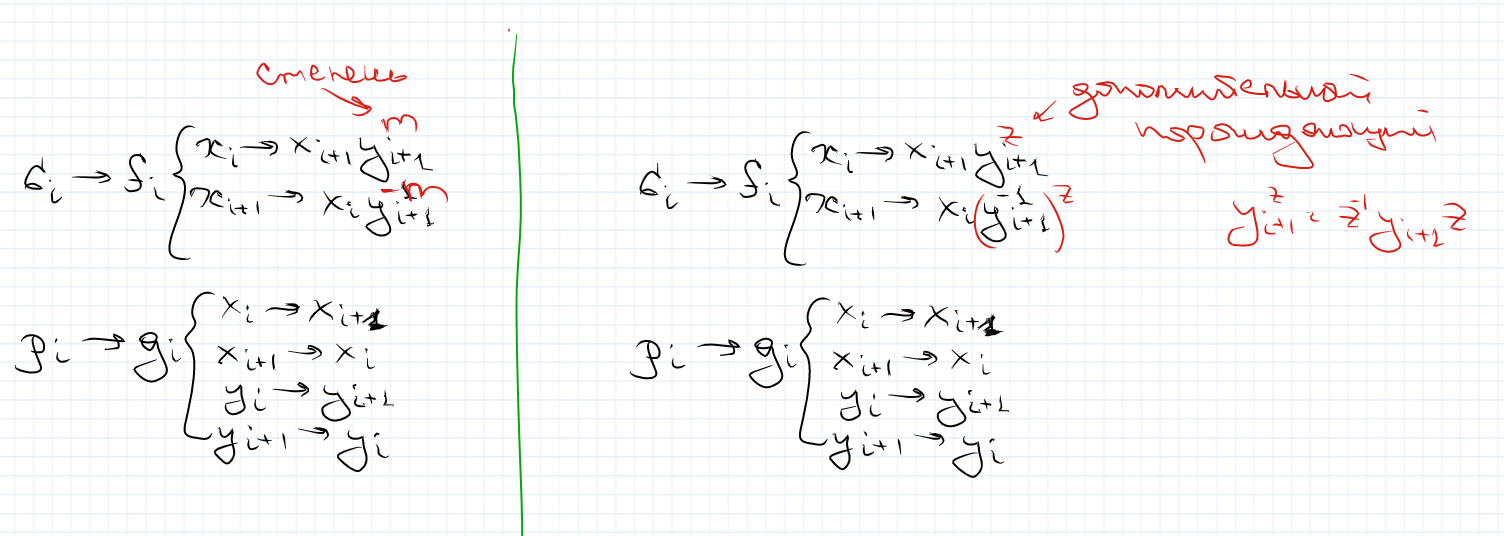
\includegraphics[width=110mm]{variant1.png}
     \item 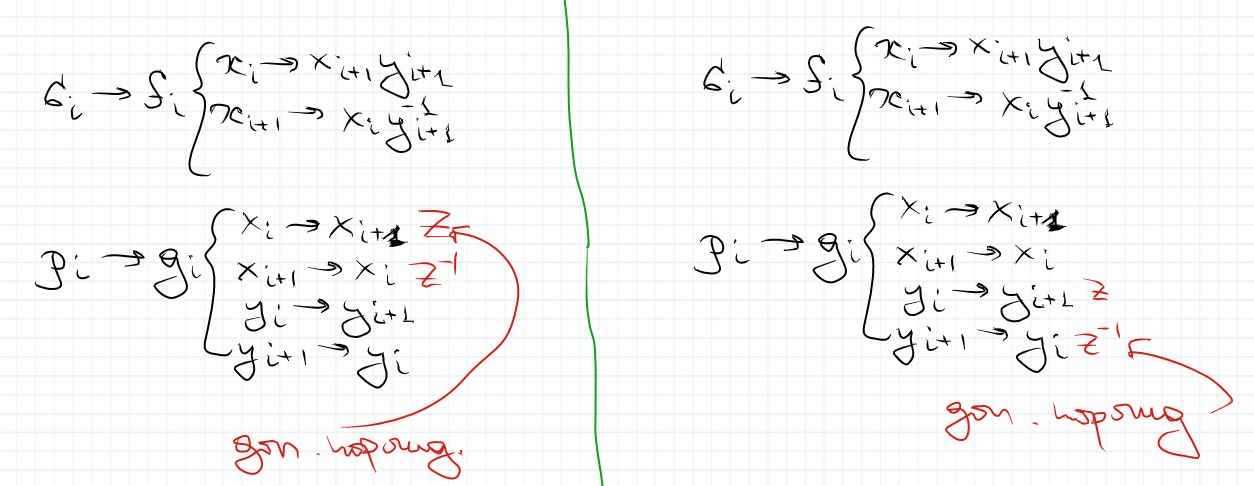
\includegraphics[width=110mm]{variant2.png}
      \item 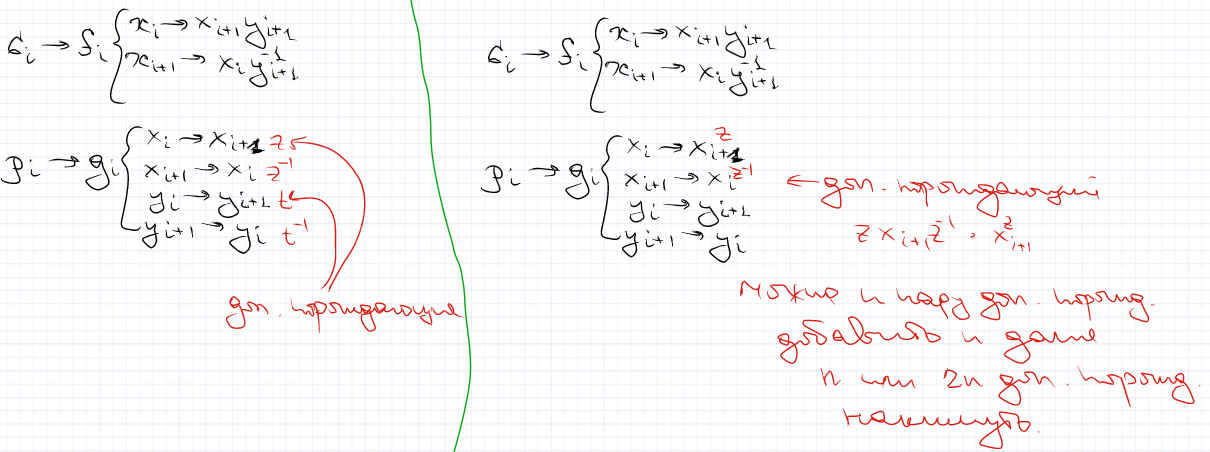
\includegraphics[width=110mm]{variant3.png}
\end{enumerate}
Most likely (up to my opinion) the map in the second line on the left is the representation. And this representation is better than the previous one (need to check).

Denote by $H_1$ the subgroup of $FVP_3=\langle a,b,c~|~[a,c]=1\rangle$ generated by the elements $a^3,b^2,c^3$. Find the intersection of $ker{\theta}$ with $H_1$. Is it trivial?

Denote by $H_2$ the subgroup of $FVP_3=\langle a,b,c~|~[a,c]=1\rangle$ generated by the elements $ac,b^2,c^3$. Find the intersection of $ker{\theta}$ with $H_2$. Is it trivial?

Denote by $H_3$ the subgroup of $FVP_3=\langle a,b,c~|~[a,c]=1\rangle$ generated by the elements $ac,b^2,a^3$. Find the intersection of $ker{\theta}$ with $H_3$. Is it trivial?

I choose $H_1,H_2,H_3$ in this way since the images of the elements which generate $H_1,H_2,H_3$ fix the elements $y_1,y_2,y_3$. 

Let $\alpha=(\rho_1\sigma_2)^6$, and let $x$ be an element from $VB_3$ (for example, $x=\rho_2$). Let $A$ be a subgroup in $VP_3$ generated by by two elements $\alpha$, $\beta=x^{-1}\alpha x$. Is it clear that this subgroup belongs to $ker(\theta)$. What can we say about this subgroup? Is it free? Can we compare it with the whole group $ker(\theta)$?

Can one reduce the dimension of the linear representation we got? I believe that it is possible and not difficult. The image of our linear representation acts on the vector space $V$ with the basis $e_1,e_2,e_3,q_1,q_2,q_3$. Look to the subspace $U$ generated by $e_1+e_2+e_3$, $q_1+q_2+q_3$. This subspace is invariant under $\theta(FVB_n)$. Look to the representation induced by $\theta$, which maps like $FVB_n\to GL(V/U)$.

Look to the kernel thinking about generators $\sigma_1, \sigma_2, \rho_1\sigma_1,\rho_2\sigma_2$. The first two generators move only the elements $x_1,x_2,x_3$, the second two generators move only the elements $y_1,y_2,y_3$.
\bibliographystyle{alpha}
\begin{thebibliography}{00}
\bibitem{problems}
R.~Fenn, D.~Ilyutko, L.~Kauffman, V.~Manturov, Unsolved problems in virtual knot theory and combinatorial knot theory, ArXiv:math/1409.2823.
\bibitem{BarBelDom}
V.~Bardakov, P.~Bellingeri, C.~Damiani, Unrestricted virtual braids, fused links and other quotients of virtual braid groups, J. Knot Theory Ramifications, V.~24, N.~12, 2015, 1550063.
\end{thebibliography}
\end{document}
